\documentclass{beamer}
\usepackage{handout}
\title{PS-1006: Politics}
\author{Tom T. Hsiao}
\date{\today}
\begin{document}
\fontspec{Times New Roman}
\begin{frame}
\begin{center}
\Large{Chapter 2 The Political System} \\
\vspace{3em}
\normalsize{Instructor: Tzu-Chi Hsiao} \\
\vspace{3em}
\small{Department of Political Science} \\
\vspace{1em}
\small{National Taiwan University} \\
\end{center}
\end{frame}
\begin{frame}{Cabinet System}
\begin{center}
  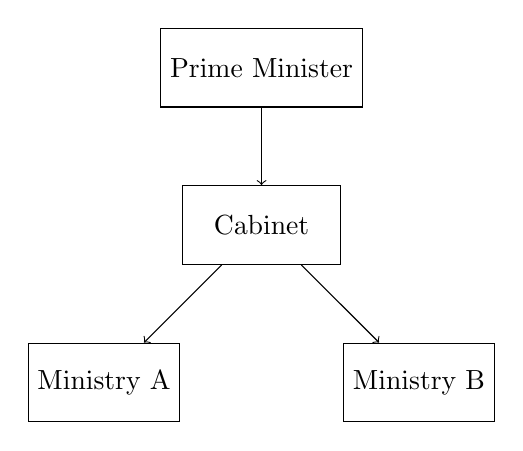
\begin{tikzpicture}[node distance=2cm]
    \node[rectangle, draw, minimum width=2cm, minimum height=1cm] (pm) at (0,0) {Prime Minister};
    \node[rectangle, draw, minimum width=2cm, minimum height=1cm] (cabinet) at (0,-2) {Cabinet};
    \node[rectangle, draw, minimum width=1.5cm, minimum height=1cm] (ministry1) at (-2,-4) {Ministry A};
    \node[rectangle, draw, minimum width=1.5cm, minimum height=1cm] (ministry2) at (2,-4) {Ministry B};
    \draw[->] (pm) -- (cabinet);
    \draw[->] (cabinet) -- (ministry1);
    \draw[->] (cabinet) -- (ministry2);
  \end{tikzpicture}
\end{center}
\begin{center}
Figure I: An example of Cabinet System.
\end{center}
\end{frame}
\begin{frame}{}
\begin{center}
\Large{End of Chapter 2}
\end{center}
\end{frame}
\end{document}
